\documentclass{article}
\usepackage[spanish]{babel}   
\usepackage[numbers,sort&compress]{natbib}
\usepackage{float}
\usepackage{listings}
\usepackage{graphicx} 	% Nos permite importar imagenes 
\usepackage{subfigure}
\usepackage[left=3cm,right=3cm,top=3cm,bottom=3cm]{geometry}

%-------------------------- Por si se romple la URL --------------------------
\usepackage[hyphens]{url}
\usepackage[hidelinks]{hyperref}
\hypersetup{breaklinks=true}	
\urlstyle{same}
\usepackage{cite}
%-------------------------- Por si se romple la URL --------------------------

\title{Reporte Tarea 12}
\author{Victor Alejandro Oviedo Martínez}



\begin{document}
\maketitle
\hrule

\section{Introduccón}\label{intro}
Para esta doceava tarea \citep{DRA.P12} se ha estudiado el tema Red Neuronal, el cual será utilizado para el reconocimiento de dígitos en imágenes en blanco y negro con tamaño $3 \times 5 $ pixeles.

\section{Desarrollo}

Para esta doceava tarea se ha planteado el siguiente problema: Estudia de manera sistemática el desempeño de la red neuronal en términos de su puntaje F (F-score) para los diez dígitos en función de las tres probabilidades asignadas a la generación de los dígitos (ngb), variando a las tres en un experimento factorial adecuado.\\

Para el desarrollo de esta tarea se a utilizado el código ejemplo proporcionado por \citet{DRA.Code}, el cual tiene el propósito de generar y entrenar una red neuronal capaz de reconocer números con un rango de 0 hasta 9, en imágenes en blanco y negro con tamaño $3 \times 5 $ pixeles. Cómo respuesta, el código \citep{DRA.Code}  devuelve una matriz de confusión de la cual se puede obtener la precisión de la red neuronal para cada imagen evaluada. Por lo tanto, se toma la información de esta matriz y se obtiene el $puntaje$ $F$ de cada número, dado que esta red neuronal evalúa el rango (0-9), obtendremos 10 $puntajes$ $F$ luego promediarlos y por lo tanto obtener el $puntaje$ $F$ de la red neuronal con las probabilidades (n, g, b) asignadas.\\

Iniciando la edición del código \citep{DRA.Code}, este es puesto en la función \texttt{simu(N, G, B)} con la finalidad de repetir su función, pero con diferentes probabilidades (n, g, b). Dentro de esta función se agregó el código necesario para calcular el $puntaje$ $F$ de la red neuronal, por lo que el resultado que entrega la función será el $puntaje$ $F$ de la red neuronal.\\


\begin{lstlisting}[language=Python]
f1 = []
    for x in range(len(contadores)):
        for y in range(len(contadores[0])):
            if x == y:
                tp = contadores[x][y]
                precision = tp / sum(list(c.iloc[x]))
                recall = tp / sum(list(c.iloc[:, x]))

                f1.append(2 * ((precision * recall) / (precision + recall)))

    F1 = np.nansum(f1) / len(f1)

    return F1
\end{lstlisting}

Para el experimento factorial se utilizaran tres instancias ya conocidas con tres probabilidades diferentes: \texttt{N = [0.95, 0.6, 0.3]}, \texttt{G = [0.92, 0.5, 0.2]}, \texttt{B = [0.002, 0.4, 0.1]}, por lo tanto se tendrán 27 resultaods diferentes. Este procedimiento será repetido 6 veces.\\

\begin{lstlisting}[language=Python]
N = [0.95,0.6,0.3]
G = [0.92,0.5,0.2]
B = [0.002,0.4,0.1]

rep = 6

for r in range(rep):
    SIMU = []
    for n in N:
        for g in G:
            for b in B:
                print()
                print('---',n,',', g,',', b,'---')
                SIMU = simu(n,g,b)
                print(SIMU)

                if r == 0:
                    simus.append(SIMU)
                if r == 1:
                    simus2.append(SIMU)
                if r == 2:
                    simus3.append(SIMU)
                if r == 3:
                    simus4.append(SIMU)
                if r == 4:
                    simus5.append(SIMU)
                if r == 5:
                    simus6.append(SIMU)
                print('---',n,',', g,',', b,'---')
                print()
\end{lstlisting}

Por último se guardan los resultados en un data frame para posteriormente graficar los resultados en un diagrama de caja.\\ 
\section{Conclusión}

En la figura \ref{f1} se puede observar los resultados de la simulación. 

\begin{figure}[H]
\begin{center}
	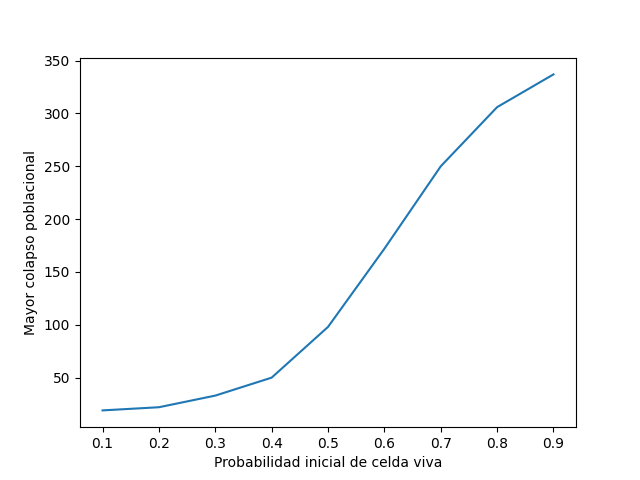
\includegraphics[height=3.5in]{/Users/victor/Desktop/Figure_1.png}
	\caption{ Simulación Combinaciones contra F-score, 6 repeticiones.}
	\label{f1}
\end{center}
\end{figure}

Cómo conclusión, observando los resultados de la figura \ref{f1}, podemos darnos cuenta que la respuesta de la red neuronal es proporcional a qué tan buenos son los datos introducidos. Tomando en cuenta que la instancia optima sería en donde; \texttt{n} = 1 y \texttt{b} = 0, y la peor; \texttt{n} = 0 y \texttt{b} = 1, no se ha agregado la probabilidad \texttt{g} dado que no demuestra una relevancia importante, ejemplo de esto se tiene la comparación en las combinaciones (0.95, 0.92, 0.002), (0.95, 0.5, 0.002), (0.95, 0.2, 0.002) con posición 1,4,7 respectivamente en la figura \ref{f1}, ya que su F-score es similar. Dado a que no se han agregado más porcentajes a la instancia \texttt{b}  y los dados no son muy variados, no es posible del todo darnos cuenta la importancia de \texttt{b}. Sin embargo podemos darnos cuenta de la importancia de \texttt{n} cuando comparamos las combinaciones donde; \texttt{n} = 0.95 contra las combinaciones donde; \texttt{n} != 0.95, el ejemplo mas notorio seria comprar la combinación (0.95, 0.92, 0.002) contra (0.6, 0.92, 0.002) en donde la primera combinación tiene una media superior a 0.7 en F-score y la segunda tiene una media aproximadamente de 2.5 en F-score, tomando en cuenta que la única diferencia entre ellos es \texttt{n} podemos ver la importancia que en ellos resulta.

%-------------------------- Por si se rompe la URL --------------------------
\Urlmuskip=0mu plus 1mu\relax
%-------------------------- Por si se rompe la URL --------------------------
\bibliography{ref.Tarea12.bib}
\bibliographystyle{plainnat}

\end{document}